%!TEX TS-program = pdflatex 
%% for textmate acceleration only

\documentclass[letterpaper]{article}
\usepackage{iccc}

\usepackage{times}
\usepackage{helvet}
\usepackage{courier}
\setcounter{secnumdepth}{0}
 
\usepackage{graphicx}
\usepackage{latexsym}
\usepackage{amssymb}
\usepackage{amsmath}
\usepackage{euscript}
%\usepackage[round]{natbib}
\usepackage[square]{natbib}
\usepackage{lstsemantic}
\lstloadlanguages{dolText}
\lstset{basicstyle=\ttfamily\footnotesize,columns=fixed}
\usepackage[hide]{ed/ed}

%\ecaisubmission   % inserts page numbers. Use only for submission of paper.
                  % Do NOT use for camera-ready version of paper.


%\setlength{\parindent}{0in}
%\linesprea
%\setlength{\parskip}{1.5pt}
%\usepackage[compact]{titlesec}
%\addtolength{\voffset}{-5mm}
%\addtolength{\hoffset}{-2mm}
%\addtolength{\textwidth}{2mm}
%\addtolength{\textheight}{2mm}	

%%%% our defs %%%%

\usepackage[T1]{fontenc}

\usepackage{color,xspace}
\usepackage{setspace}
%\usepackage{diagrams}
%\newarrow{Dotsto} ....>
%\newarrow{Line} -----

\usepackage{tabularx}

%% local definitions
\newcommand{\Dolce}{\textmd{\textsc{Dolce}}\xspace}
\newcommand{\OWL}{\textmd{\textsc{OWL}}\xspace}
\newcommand{\hOWL}{\textmd{\textsc{DOL-OWL}}\xspace}
\newcommand{\CASL}{\textmd{\textsc{Casl}}\xspace}
\newcommand{\HetCASL}{\textmd{\textsc{HetCasl}}\xspace }
\newcommand{\Hets}{\textmd{\textsc{Hets}}\xspace}
\newcommand{\SROIQD}{\ensuremath{\mathcal{SROIQ}(D)}\xspace}
\newcommand{\Econn}{\mbox{$\mathcal{E}$-con}\-nec\-tion\xspace}
\newcommand{\EConn}{\mbox{$\mathcal{E}$-Con}\-nec\-tion\xspace}
\newcommand{\Econns}{\mbox{$\mathcal{E}$-con}\-nec\-tions\xspace}
\newcommand{\EConns}{\mbox{$\mathcal{E}$-Con}\-nec\-tions\xspace}
\newcommand{\Econd}{\mbox{$\mathcal{E}$-con}\-nec\-ted\xspace}
\newcommand{\DDL}{\ensuremath{\textrm{DDL}}\xspace}
\newcommand{\DDLs}{\ensuremath{\textrm{DDLs}}\xspace}
\newcommand{\Sconn}{\mbox{$\mathcal{S}$-con}\-nec\-tion\xspace}
\newcommand{\SConn}{\mbox{$\mathcal{S}$-Con}\-nec\-tion\xspace}
\newcommand{\Sconns}{\mbox{$\mathcal{S}$-con}\-nec\-tions\xspace}
\newcommand{\SConns}{\mbox{$\mathcal{S}$-Con}\-nec\-tions\xspace}
\newcommand*{\DOL}{\ensuremath{\mathsf{DOL}}\xspace}

\newcommand{\Mod}{\mathbf{Mod}}
\newcommand{\forget}[1]{|_{#1}}

\newcommand{\parrow}{\longrightarrow\!\!\!\!\!\!\!\!\circ \hspace{0.2 cm}}


%% Theorems

%\theoremstyle{plain}
\newtheorem{theorem}{Theorem}
\newtheorem{lemma}[theorem]{Lemma}
\newtheorem{corollary}[theorem]{Corollary}
\newtheorem{proposition}[theorem]{Proposition}
\newtheorem{example}[theorem]{Example}
\newtheorem{observation}[theorem]{Observation}
\newtheorem{claim}[theorem]{Claim}
\newtheorem{fact}[theorem]{Fact}

%\theoremstyle{definition}
\newtheorem{definition}[theorem]{Definition}
%\theoremstyle{remark}
\newtheorem{remark}[theorem]{Remark}


%%% Alignments
%% 
\newcommand{\Va}{\ensuremath{\mathsf{V}}}
\newcommand{\Wa}{\ensuremath{\mathsf{W}}}
\newcommand{\Ma}{\ensuremath{\mathsf{M}}}
\newcommand{\La}{\ensuremath{\Lambda}}
\newcommand{\Da}{\ensuremath{\mathsf{X}}}


%\usepackage[mtplusscr,mtbold]{mathtime}

%
\newcommand{\defsty}[1]{\textbf{#1}}
\newcommand{\weg}[1]{}
\newcommand{\oliver}[1]{{\bf{\textsc{OK:~}{[\textit{#1}]}}}}
\newcommand{\till}[1]{{\bf{\textsc{TM:~}{[\textit{#1}]}}}}
\newcommand{\joana}[1]{{\bf{\textsc{JH:~}{[\textit{#1}]}}}}
\newcommand{\john}[1]{{\bf{\textsc{JB:~}{[\textit{#1}]}}}}

%% blending definitions

\newcommand{\blend}{\ensuremath{\mathfrak{B}}\xspace}
\newcommand{\base}{\ensuremath{\mathcal{B}}\xspace}
\newcommand{\Sig}[1]{\ensuremath{\mathsf{Sig}}(#1)}
\newcommand{\Ax}[1]{\ensuremath{\mathsf{Ax}}(#1)}
\newcommand{\clos}[1]{\ensuremath{\mathsf{clos}}(#1)}
\newcommand{\con}[1]{\ensuremath{\mathsf{#1}}} % from DL package
\newcommand{\auf}{\left\langle}
\newcommand{\zu}{\right\rangle}

%%%% 

\definecolor{orange}{cmyk}{0,0.56,0.87,0}
\newtheorem{task}{\color{orange} 
\textbf{\underline{Task}}}
\newtheorem{tof}{\color{red} 
\textbf{\underline{True or False?}}}

\usepackage{graphicx}

\usepackage{url}
%\usepackage[pdftitle={},pdfauthor={},linkbordercolor=white,pdffitwindow=true]{hyperref}

%%%%

\pdfinfo{
/Title (Fabricating Monsters is Hard. Towards the Automation of Conceptual Blending)
/Subject (Proceedings of ICCC)
/Author (Mihai Codescu, Maria Hedblom, Eugen Kuksa, Ewen Maclean, Till Mossakowski, Fabian Neuhaus, Marcus Pinnecke)}
\title{Fabricating Monsters is Hard\\ Towards the Automation of Conceptual Blending}
%\title{Manufacturing Monsters\\ \LARGE Blending the Lionman and other Curious Creatures\\ length = 6 + 1 for refs}

%\subtitle{A Formal Model with DOL}

\setlength\titlebox{2.8in}
\author{
Maria Hedblom \and Till Mossakowski \and Fabian Neuhaus \and Marcus Pinnecke\\
Institute for Cooperating Intelligent Systems,  Otto-von-Guericke University of Magdeburg, Germany
\AND
Mihai Codescu \and Oliver Kutz \\
Free University of Bozen-Bolzano, Italy
\AND
Eugen Kuksa \\
Department of Computer Science, University of Bremen, Germany
\AND
Ewen Maclean\\
Centre for Intelligent Systems and their Applications, University of Edinburgh, UK}

\begin{document}





\maketitle



\begin{abstract}
The theory of conceptual blending has been applied very successfully  in cognitive
 science to explain the process of concept generation. In previous work, we have shown
  a formalisation and implementation of conceptual blending that is borrowing techniques 
  from logic, ontological engineering, and algebraic specification. However, so far 
  our attempts (and similar approaches in the literature) have been reconstructive;
   that is they show how a particular concept (e.g., houseboat)  can be `discovered' 
   by computationally blending two carefully selected input spaces (e.g, a house and a boat) 
   and a suitable base. This paper describes an attempt to take the next step and automate the
    concept generation based on a database of input spaces. Particularly, we attempt to create monsters from a library of animals formalised as OWL ontologies.
 
%We introduce ontological blending as a method for combining ontologies. Compared with existing combination techniques that aim at integrating or assimilating categories and relations of thematically related ontologies, \emph{blending} aims at creatively generating (new) categories and ontological definitions; this is done on the basis of input ontologies whose domains are thematically distinct but whose specifications share structural or logical properties. As a result, ontological blending can generate new ontologies and concepts and it allows a more flexible technique for ontology combination compared to existing methods. 
%
%\noindent Our approach to computational creativity in conceptual blending is inspired by methods rooted in cognitive science (e.g., analogical reasoning), ontological engineering, and algebraic specification. Specifically, we introduce the basic formal definitions for ontological blending, and show how the distributed ontology language \DOL (currently being standardised within the OntoIOp---Ontology Integration and Interoperability---activity of ISO/TC 37/SC 3) can be used to declaratively specify blending diagrams. %, and analogical reasoning in particular.
%%\textbf{max: 6 pages; abstract deadline: 15 February 2010; paper deadline: 22 February 2010}\\
%% and based on structural blending in narrative generation. ...
%%% 
%\weg{Research on approaches, techniques, and their implications for relating different ontologies have become one of the central research topics in ontology engineering today. Such methods range from matching, mapping, and merging to aligning, bridging, and connecting different or similar ontologies, their single categories, or relations. However, such approaches often presuppose that ontologies may consistently exchange information between each other, i.e., that consistent links between each other's categories or relations can be established, and that the ontologies more or less specify the same topic, only from different perspectives. 
%%% 
%In contrast to this more eclectic `uniting view' on relating ontologies, they can also be seen as, potentially mutually contradicting or simply complementing, contributors that may be merged into a new ontology specification of a newly created topic which emerges from a `creative' blend of the two specifications. 
%%% %in particular, that there is one ``right'' way of specifying certain topics/information.
%In this case, \emph{ontological blending} can be the best choice, as introduced and discussed in this paper.}
\end{abstract}

\section{Introduction}

Conceptual blending in the spirit of Fauconnier and Turner operates by
combining two input `conceptual spaces', construed as rather minimal
descriptions of some thematic domains, in a manner that creates new
`imaginative' configurations \citep{FauconnierTurner2003,Turner2014}. A classic example for this is the
blending of the concepts \emph{house} and \emph{boat}, yielding as
most straightforward blends the concepts of a \emph{houseboat} and a
\emph{boathouse}, but also an \emph{amphibious vehicle}. These examples
 illustrate that, typically, the blended spaces inherit some features from
  either space and combine them to something novel. The blending of the input 
spaces involves a base space, which contain shared structures between both input spaces. 
The structure in the base space is preserved in the blended space (the \emph{blendoid}). 

Goguen defines an approach that he terms \emph{algebraic semiotics} in 
 which certain structural aspects of semiotic systems are logically
  formalised in terms of algebraic theories, sign systems, and their mappings \citep{Goguen99}. 
%
In \cite{goguenharrell10}, algebraic
semiotics has been applied to user interface design and conceptual blending.
 Algebraic semiotics does not claim to provide a comprehensive formal theory of blending 
 -- indeed, Goguen and Harrell admit that many  aspects of blending, in particular concerning
  the meaning of the involved notions, as well as the optimality principles for blending, 
  cannot be captured formally.  However, the structural
aspects \emph{can} be formalised and provide insights into the space of possible blends. 
The formalisation of these blends can be formulated  using the algebraic specification language OBJ3 \citep{GoguenMalcolm96}. 


In \cite{HoisEtAl2010,blendingc3gi12,iccc14-ontohub}, we have presented an approach to computational conceptual blending,  which is in the tradition of Goguen's proposal. In these earlier papers, we suggested to represent the input  spaces as ontologies (e.g., in the OWL Web Ontology Language\footnote{With `\OWL' we refer \ to \OWL 2 DL, see \url{http://www.w3.org/TR/owl2-overview/}}). We moreover presented how  the Distributed Ontology Language (DOL) can be used to specify conceptual blends with the help
  of \emph{blending diagrams}. These diagrams encode the relationships between the base space 
  and the (two or more) input spaces. These \emph{blending diagrams} can be executed by Hets,
  \ a proof management system. Hets is integrated into Ontohub,\footnote{\url{www.ontohub.org}} 
  an ontology repository which allows users to manage and collaboratively work on ontologies.  DOL, Hets, and Ontohub provide a powerful set of tools,    which make it easy to specify and computationally execute conceptual blends. 

In this paper, we will discuss how we utilised DOL, Hets, and Ontohub in an attempt to build 
a prototype system that automates concept invention. The goal is to make the step from a
 reconstructive approach, where computational conceptual blending is illustrated by blending 
 one concept (e.g., houseboat) with the help of some carefully selected input spaces
  (e.g, a house and a boat) to a system that autonomously selects two (or more) ontologies 
  from a repository in Ontohub and attempts to blend them in a way that meets some given requirements. Within the extensive literature on conceptual blending, few attempts have been made at a  (more or less) complete automation of the blending process, notable exceptions include \cite{goguenharrell10}, \cite{Pereira07}, \cite{LiEtAl2012}, and \cite{veale2000computation,Veale2012}.
  
 \medskip\noindent 
  In our experiment we use a repository of ontologies about animals as input spaces and try to blend
   them into monsters.  In the next section, we are going to discuss the underlying model 
   of our approach and how we simplified it in our prototype implementation.  Finally, we summarise our initial results and discuss future work. 

\section{The Approach}
%\subsection{The Schorlemmer Model for Computational Blending}
%\subsection{General Approach}
We follow a variation of Goguen's approach to computational conceptual blending,
which has been proposed within the COINVENT research project (see Figure \ref{blendingModel} and \url{www.coinvent-project.eu}) and summarised by Marco Schorlemmer. In the next sections we discuss the various elements of this revised blending approach which we will refer to as the \emph{Schorlemmer model}. Details of this revised model have not been published elsewhere so far, but the general background of the approach can be found in \cite{iccc14-coinvent}.

\subsection{(Weakened) Input Spaces}
 In this model there are two (or more) input spaces $I1$ and $I2$, which are in our 
 case represented as OWL ontologies.  These ontologies are randomly selected from a repository 
 of animal ontologies in Ontohub. These ontologies are not `fine-tuned' for a particular blend, 
 but represent some features of types of animals, in particular their habitat, their diet, 
 and some anatomical information (see Figure \ref{inputExample}). The goal is that in the future 
 we will be able to easily both increase the depth of information that is provided in the animal ontologies as 
 well as add new ontologies covering additional organism. 
 
 
 \begin{figure*}[htbp]
\begin{center}
%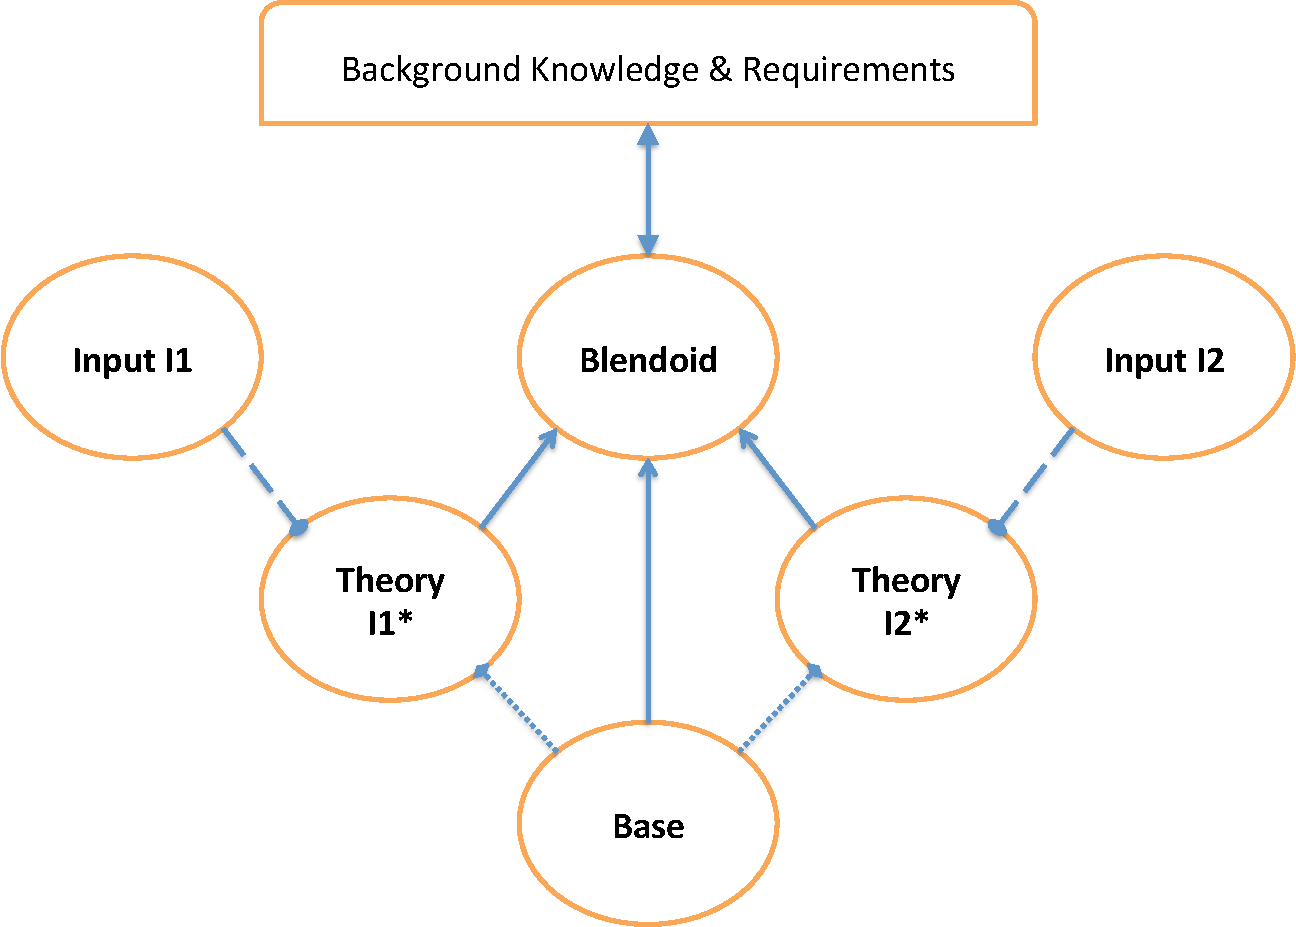
\includegraphics[width=0.7 \textwidth]{blendModel.pdf}
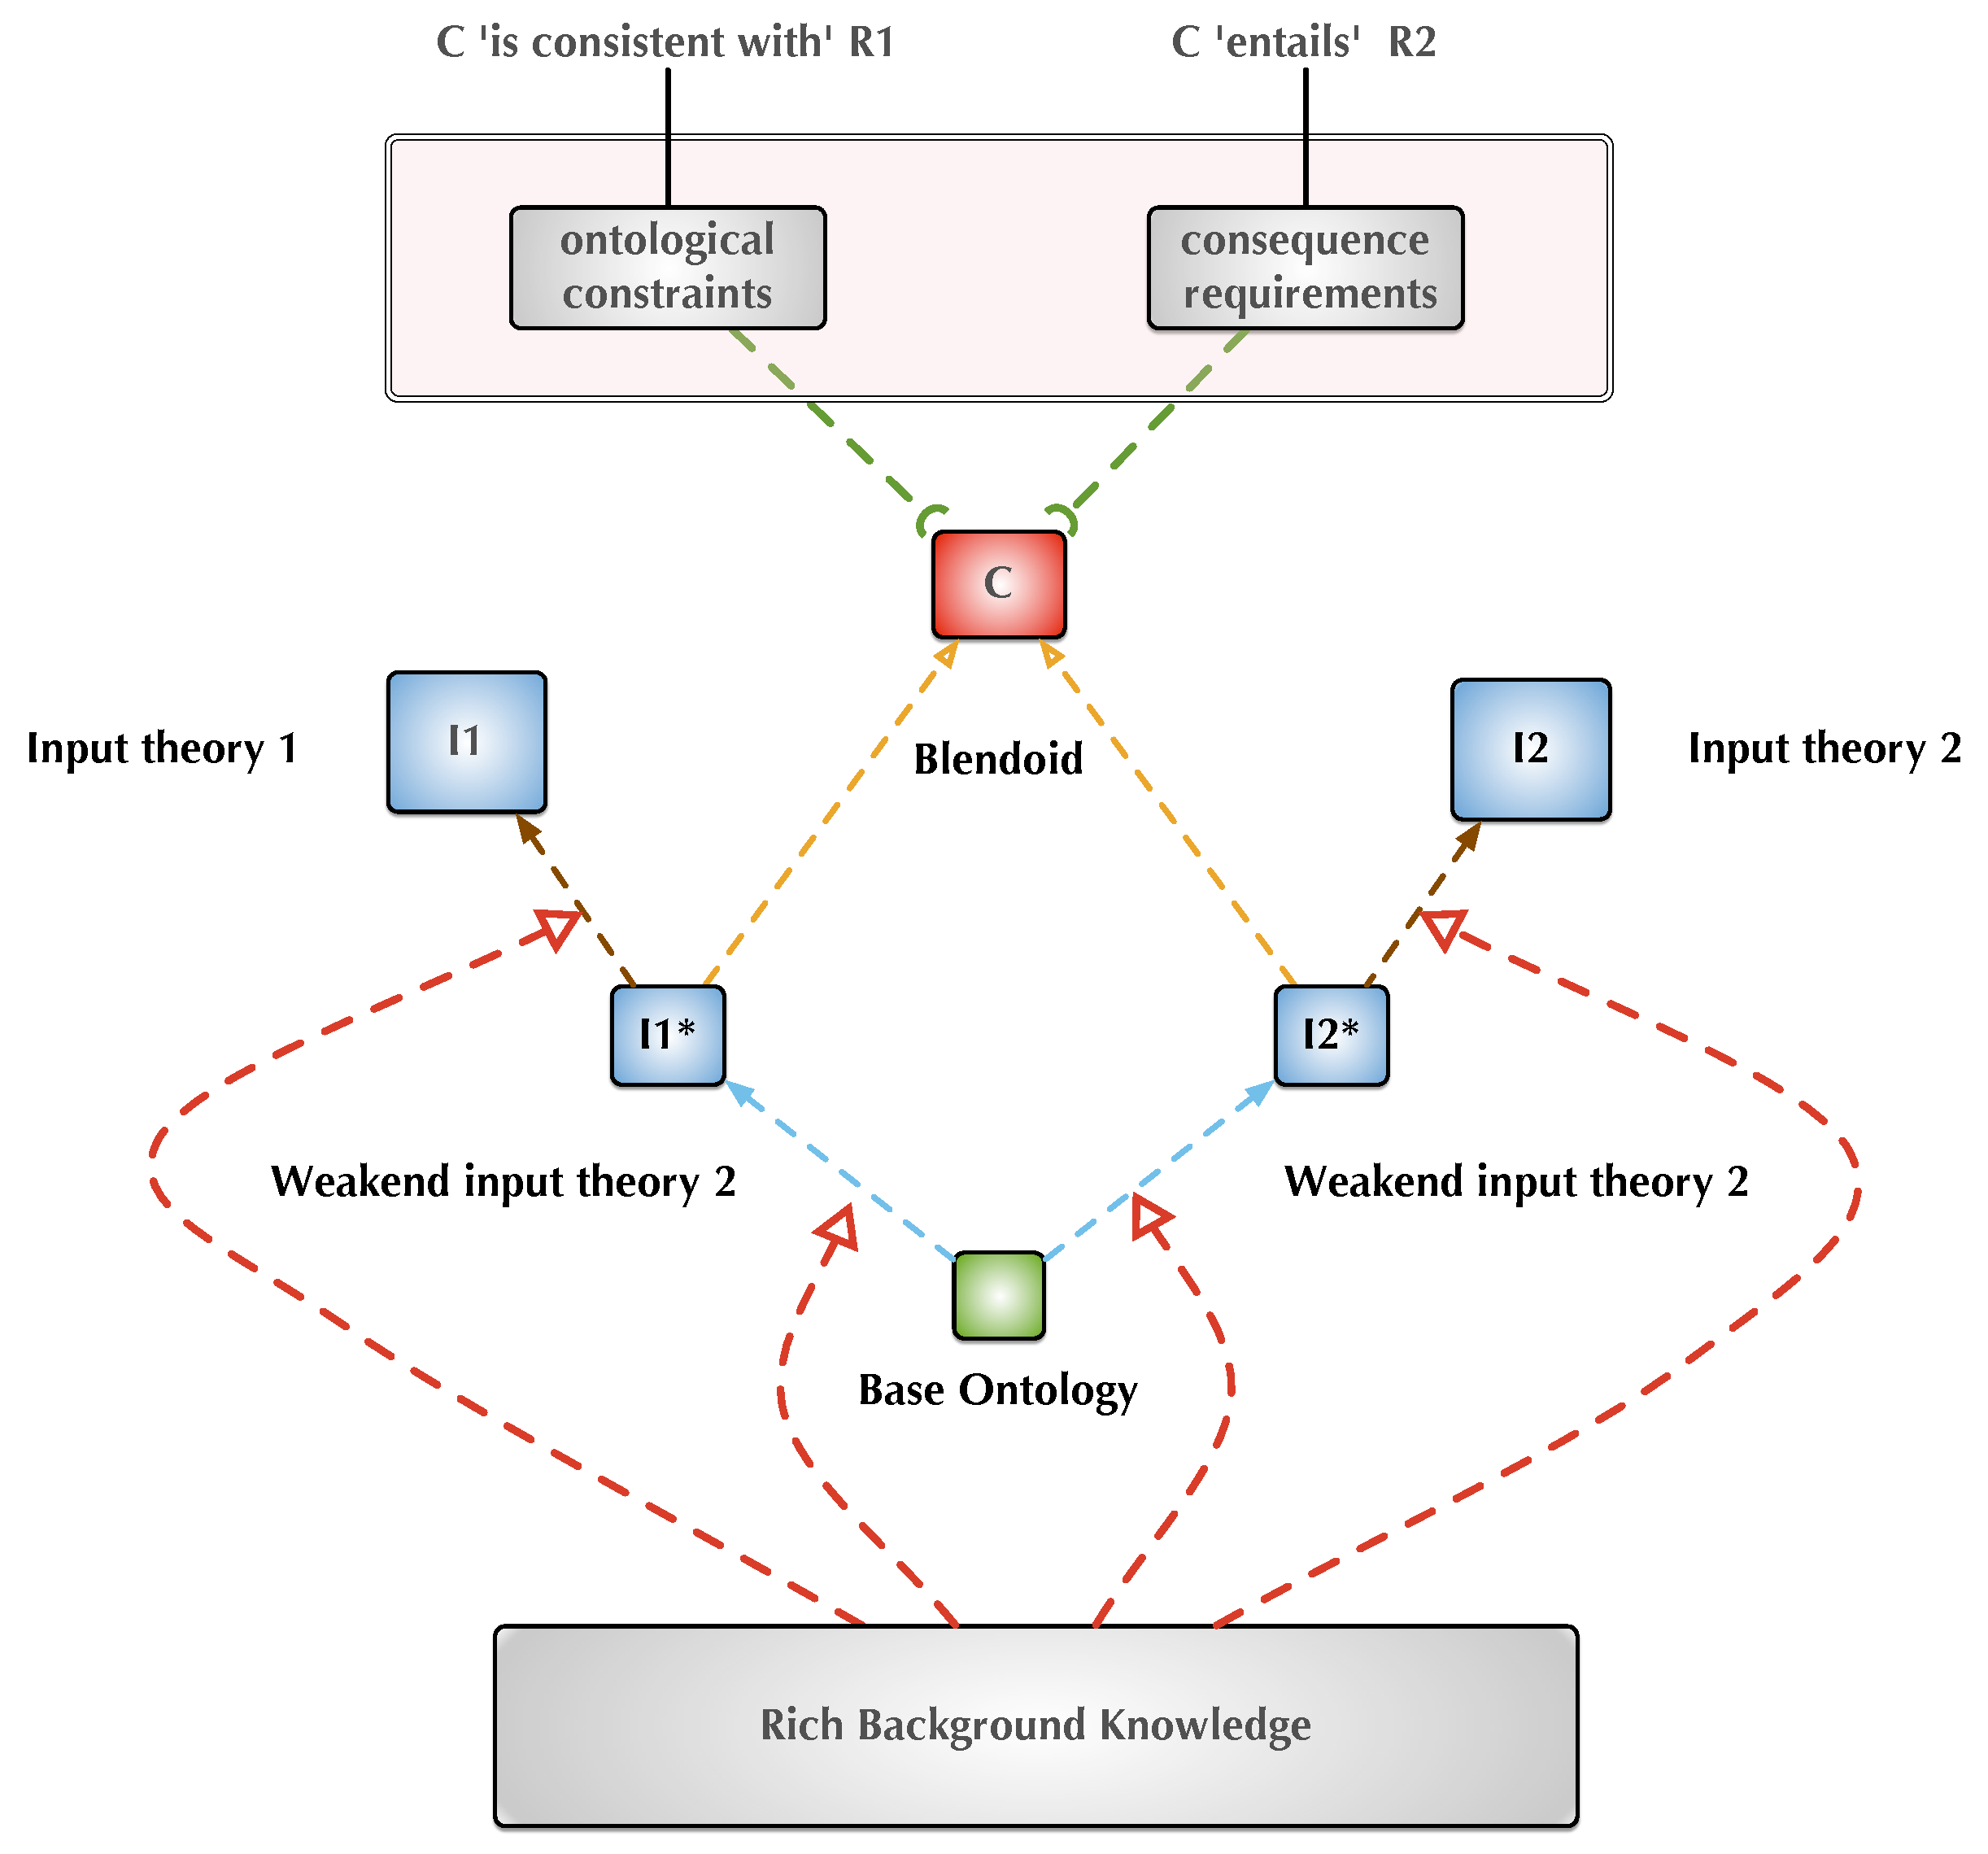
\includegraphics[width=0.9 \textwidth]{blendoids-coremodel}
\caption{The core Schorlemmer model for computational blending enriched with evaluation and background layers}
\label{blendingModel}
\end{center}
\end{figure*}

 \begin{figure}[htbp]
\begin{lstlisting}[basicstyle=\ttfamily\scriptsize,language=dolText,morekeywords={props,excluding,ObjectProperty,Class,DisjointUnionOf,SubClassOf,Characteristics,Transitive,Asymmetric,SubPropertyOf,DisjointClasses,EquivalentTo,Asymmetric,inverse,only,forall,iff,if,or,exists,bridge,distributed},escapechar=@,mathescape,alsolanguage=owl2Manchester]
Class: Tiger 
	SubClassOf: Mammal 
	SubClassOf: Carnivore 
	SubClassOf: has_habitat some Jungle 	
	SubClassOf: has_body_shape some QuadrupedShape
	SubClassOf: has_part some Fang 
	SubClassOf: has_part exactly 4 Claw
	SubClassOf: has_part exactly 1 Tail  
	SubClassOf: covered_by some Hair
	
Class: Viper
	SubClassOf: Reptile 
	SubClassOf: Carnivore 
	SubClassOf: has_habitat some 
			(Grasslands or Wetlands or Rocks)
	SubClassOf: has_body_shape some SnakeShape
	SubClassOf: has_part only (not Leg)
	SubClassOf: has_part some PoisonFang
	SubClassOf:  covered_by some Scales 	
	
\end{lstlisting}
\caption{Input space example}
\label{inputExample}
\end{figure}
\vspace{-2em}
%\ednote{what are those ... in the schorlemmer picture??}
 
The Schorlemmer model differs from the model proposed in  \cite{goguenharrell10} by introducing an extra step:
 the ontologies  $I1$ and $I2$ are not blended directly, but are first weakened to two theories 
 $I1^*$ and $I2^*$ (see Figure~\ref{blendingModel}).  There are different strategies that can be used to generate  the weaker theories
  from the input ontologies; the only constraint is that input ontologies logically entail their weakened 
  counterparts. The purpose of this extra step is to remove some of the information from the input spaces 
  that is undesired for the blend. There are several reasons why such a step might be necessary. Firstly, when blending a concept from a given ontology, typically large parts of the ontology are in fact off-topic. Logically speaking, when extracting a module for the concept in question, large parts of the ontology turn out to be logically irrelevant (module extraction is typically based on conservative extensions, see e.g.\ \cite{KLWW-ECAI-08}). Secondly, when running the blend it may become obvious that the blendoid preserved too many properties from the input spaces. In this case,  weakening the input spaces will lead to a better result. 
  
  \smallskip\noindent
  We will discuss these issues in more detail below in the context of evaluation. 

\subsection{Base and Interpretations}
The weakened input ontologies $I1^*$ and $I2^*$ are used to generate the base ontology. 
The base ontology is identifying some structure that is shared across $I1^*$ and $I2^*$.
 Or, to put it differently, the base ontology contains some theory, which can be found in
  both the input spaces, but it abstracts from the peculiarities of the input spaces and generalises the theory in some domain-independent way. 

From the perspective of the workflow the base ontology is a more general theory that
 is generated  from the (weakened) input ontologies. From a logical point of view, 
 there exist two \emph{interpretations} which embed the base ontology into  $I1^*$ 
 and $I2^*$. (In Figure \ref{blendingModel} these are represented by the thinly dotted 
 connectors between the base and  $I1^*$ and $I2^*$.) These interpretations are a key 
 element to make the automatic blending process work (see next section). 

\subsection{The Blend} 
The ontologies  $I1^*$ and $I2^*$ together with the base ontology and the two
  interpretations that connect the base to  $I1^*$ and $I2^*$ determine the blendoid. 
  Informally, what happens is that the blendoid is a disjoint union of $I1^*$ and $I2^*$, 
  where the shared structure from  the base is identified.\footnote{Technically, the 
  blendoid is the co-limit of the underlying diagram. For the formal details see \cite{AHS} and \cite{blendingc3gi12}.}

For example, assume one of our input ontologies is about tigers and the other about vipers.
 $I1^*$ and $I2^*$ are weakened versions of these input ontologies, where only some of the 
 properties of tigers and vipers, respectively, are included. If the base ontology is empty, then 
 the resulting blendoid consists of a theory that contains both tigers and snakes, but nothing is blended.
  If the base ontology identifies the tiger with the viper, the blendoid will be a monster that combines all 
  the features of tigers and vipers that have  been preserved in $I1^*$ and $I2^*$; e.g. you may get a tiger 
  with a forked tongue and scales instead of hair. A different base may identify the viper with the tail of the 
  tiger, in that case the resulting blend may consist of a tiger whose tail has eyes and poisonous fangs.

\subsection{Background Knowledge and Requirements}
To make the Schorlemmer model work in practice, the background knowledge 
and requirements have to play an essential role.  Figure \ref{blendingModel} 
represents a static view of how two input spaces are blended. However, since there are a
 vast number of potential blends, most of which are poor, computational concept blending is an iterative process.
  In each cycle, a new blendoid is created, and is evaluated against ontological constraints, i.e.\ a set $R1$ of axioms drawn from (common sense) background knowledge and with which a blendoid should not be in conflict, as well as a set  $R2$ of consequence requirements, i.e.\ a collection of desired entailments a blendoid should yield. If the blendoid is rejected according to these criteria, the next cycle is started with different weakened input spaces and/or a different base.
    Ideally, the results of the evaluation is supposed to guide the changes in the next cycle. %(in Fig.~\ref{blendingModel}, the red arrows feed the background knowledge into the choice of the respective mappings).  
    We will discuss the role of evaluation in more detail below.



\subsection{Our Initial Implementation}
For the purpose of our experiment we created a small library of ontologies
 of animals, describing some of their anatomy, their habitats, and their diets.
  Further, we developed several ontologies that contained background information. 
  All ontologies were written in OWL Manchester Syntax.

In order to automate the blending process as modelled in Figure~\ref{blendingModel}, 
we had to  provide the following functionality: given two selected ontologies from the 
repository, repeat the following steps until the blend is successful: 

\begin{description}
	\item[(i)] weaken the input spaces and generate $I1^*$ and $I2^*$, 
	\item[(ii)] create the base ontology and the  interpretations that link the base to $I1^*$ and $I2^*$,  
	\item[(iii)] execute the blend  and generate the blendoid, and
	\item[(iv)] evaluate the blendoid.  
\end{description}



\paragraph{Weakening the input space.} For the purpose of the initial implementation
 we wrote a simple script that removes some axioms in an OWL file.
  The script preserves the declaration of classes, individuals, and properties
   (thus, the signature of the ontology is not changed). 
   The selection of the axioms that are deleted is randomised.

\paragraph{Generating the base ontology.}
For the purpose of an initial implementation we are currently working with a very
 simplified approach, where the bases consist basically of the shared signature
  of $I1^*$ and $I2^*$, which allows for trivial interpretations from the base.  
  The only exception is the class Monster, which is mapped to the animals within
   the input spaces. E.g., Monster in the base ontology is mapped to the input ontologies $I1^*$ and $I2^*$, namely to Tiger and  Viper, respectively.\footnote{This approach presupposes that the 
   same terminology is used consistently across the animal ontologies. However, since
  the ontologies were all developed in-house, this was not an issue.} Figure \ref{base} shows the complete base and both interpretations for our running example.
 \begin{figure}[htbp]
\begin{lstlisting}[basicstyle=\ttfamily\scriptsize,language=dolText,morekeywords={props,excluding,ObjectProperty,Class,DisjointUnionOf,SubClassOf,Characteristics,Transitive,Asymmetric,SubPropertyOf,DisjointClasses,EquivalentTo,Asymmetric,inverse,only,forall,iff,if,or,exists,bridge,distributed},escapechar=@,mathescape,alsolanguage=owl2Manchester]
ontology base = 
	ObjectProperty: has_habitat
	ObjectProperty: has_body_shape
	ObjectProperty: has_part 
	ObjectProperty: covered_by 
	Class: Carnivore	
	Class: Monster

interpretation base2Viper: base to viper  =
	Monster |-> Viper

interpretation base2Tiger: base to tiger  =
	Monster |-> Tiger

ontology monsterblend  = 
    combine base2Viper, base2Tiger

\end{lstlisting}
\caption{Base and Interpretations}
\label{base}
\end{figure}
\vspace{-2em}


  
  While
  this approach works, it limits the number of interesting blends severely. E.g.,
  in our example of blending  Tiger with  Viper, the approach allows blendoids
 like a tiger with poisonous fangs and scales, but no tigers with a viper-like tail, 
 because this would require the base to identify the tail of the tiger with the snake. 
 This, however, can be easily obtained by allowing more complex base mappings.   

\paragraph{Running the Blend.}
 Hets provides the capability to run the blend. Technically, this is a colimit computation,  a construction that abstracts the operation of disjoint unions modulo the identification of certain parts specified by the base and the interpretations, as discussed in detail in  \cite{Goguen03semioticmorphisms,hyper2010,blendingc3gi12}.

Figure \ref{exampleBlendoid} shows an example of a blendoid that is derived from the input spaces in Figure \ref{inputExample} with a weakening of both input spaces. In this case the monster inherits most of the tiger qualities, but it has poisonous fangs and  is (partially) covered by scales. 
 \begin{figure}[htbp]
\begin{lstlisting}[basicstyle=\ttfamily\scriptsize,language=dolText,morekeywords={props,excluding,ObjectProperty,Class,DisjointUnionOf,SubClassOf,Characteristics,Transitive,Asymmetric,SubPropertyOf,DisjointClasses,EquivalentTo,Asymmetric,inverse,only,forall,iff,if,or,exists,bridge,distributed},escapechar=@,mathescape,alsolanguage=owl2Manchester] 
Class: Monster
       SubClassOf: Carnivore
       SubClassOf: has_part some PoisonFang
       SubClassOf: covered_by some Scales
       SubClassOf: Mammal
       SubClassOf: has_habitat some Jungle
       SubClassOf: has_body_shape some QuadrupedShape
       SubClassOf: has_part some Fang
       SubClassOf: has_part exactly 4 Claw
       SubClassOf: has_part exactly 1 Tail
       SubClassOf: covered_by some Hair 
\end{lstlisting}
\caption{Example Blendoid}
\label{exampleBlendoid}
\end{figure}
\vspace{-2em}
  
\paragraph{Evaluation.}  \label{eval}
 Hets integrates a number of theorem prover and consistency checkers. 
 We used Pellet and Darwin for the evaluation of the blendoids. 
 
 
We evaluate blendoids both by considering its internal consistency and 
by looking for potential clashes with our background knowledge. For this purpose 
we use DOL to specify a new ontology that combines a blendoid with the background knowledge. 
This combined ontology is evaluated for logical consistency via Hets.  
The reason why the background knowledge is essential here is that   the detection of problems 
often requires more information than is contained within the blendoid.
 To return to our example about tigers and vipers, assume  
the input spaces in Figure \ref{inputExample} were weakened and that 
 $I1^*$ 
 contains the information that tigers have four claws,  and $I2^*$ contains
  the information that vipers have no legs. In this case, the resulting
   blend will be a leg-less monster with claws. Without the additional background 
   knowledge that claws are part of legs, it is impossible for a consistency checker to detect the inconsistency.  

One requirement for a good blendoid is that it needs to combine information from 
both input spaces. In other words, if the information in the blendoid is contained
 in one of the input ontologies, then the blendoid is not a good conceptual blend. 
 Since our approach involves a weakening of the input ontologies, it may happen 
 that one of the ontologies is weakened so extremely that it does not contribute   
 anything significant to the blendoid. 


Often, a blending process is done with certain requirements in mind. E.g., 
in our example we may look for monsters that have four appendages. 
These requirements can be stated in DOL as proof obligations that have to 
be proven from the blendoid together with the background knowledge. 


\section{Discussion and Future Work}

Our prototype implementation works in the sense that the system creates monsters by blending two animals.
 It works, in spite of the fact that two essential components of the blending model are handled quite bluntly: 
 
 \begin{description}
\item[(i)] the base space is fixed to the shared signatures of the weakened input spaces and, thus,  trivial; and
\item[(ii)] the weakening of the input spaces does not utilise the results of the evaluation, but happens randomly. 
\end{description}

We here  focused on making the workflow work, while accepting that some modules within the workflow are trivialised. 
Future work includes refining such a workflow, and of course using more sophisticated methods for its various parts. 

Firstly, regarding the generation of the base ontology, we are planning to use heuristic-driven theory projection (HDTP) as outlined in \cite{Martinezetal2011,schweringEtAl09}. Taking $I1^*$ and $I2^*$ as input theories, HDTP  applies anti-unification techniques to generalise the input ontologies to a more general theory. So far, HDTP has been implemented for a sorted version of FOL. To make it work in our context, we are going to need to support OWL directly (the preferred approach) or reduce OWL anti-unification to FOL anti-unification (e.g.\ via using a logic translation first and then a theory projection).  

Secondly, regarding weakening of theories, we particularly plan to use the idea of `amalgams' as proposed in \cite{ontanon2010amalgams}. 

Thirdly, regarding revision of inconsistent blendoids, a number of tools and approaches are available to be employed in this context, amongst them: non-monotonic reasoning, in particular belief revision \citep{Alchourron85a}, and ontology debugging techniques, in particular for OWL \citep{Kaly05}. Indeed, ontology debugging techniques are readily available via the OWL API.\footnote{See \url{http://owlapi.sourceforge.net}} %\ednote{check and refine}. 
%However, in the case of blending....\ednote{specifics of blending, number of calls for consistency checks, ...}

 Concerning the latter, a promising idea is to interactively generate competency questions (cf.\ \cite{gruninger1995role,ren2014towards}) from justifications for inconsistencies \citep{Kalyanpur:2007:Finding}. Here, a user can steer the generation of new blends by rejecting certain ways to fix an inconsistent blendoid. A similar debugging workflow has recently been proposed by \cite{intontdebug14}, although only for the debugging of single inconsistent ontologies. In the case of blending, such approaches need to be adapted to a revision procedure covering networks of ontologies, where several ontologies (i.e.\ input and base ontologies) as well as the mappings between them are subject to revision.



% Concept schemas

% Believe revision, OWL debugging


While our system works, it often does not produce very  good monsters. 
Interestingly, the limitations of the results are not (or only indirectly) caused
 by the fixing of the base space or the randomised weakening of the input spaces. 
 For example, consider the result of the blend of a shark and a horse in Figure \ref{outputExample}. 
 The monster in this ontology has  fins and a tail,  it is a  herbivore and  lives in some grasslands. 
 \begin{figure}[htbp]
\begin{lstlisting}[basicstyle=\ttfamily\scriptsize,language=dolText,morekeywords={props,excluding,ObjectProperty,
Class,DisjointUnionOf,SubClassOf,Characteristics,Transitive,Asymmetric,SubPropertyOf,
DisjointClasses,EquivalentTo,Asymmetric,inverse,only,forall,iff,if,or,exists,
bridge,distributed},escapechar=@,mathescape,alsolanguage=owl2Manchester]
Class: Monster
	SubClassOf: Herbivore 
	SubClassOf: has_habitat some Grassland
	SubClassOf: has_part some Fin 
	SubClassOf: has_part exactly 1 Tail  
\end{lstlisting}
\caption{Poor Blendoid}
\label{outputExample}
\end{figure}
\vspace{-2em}

The ontology in Figure \ref{outputExample} illustrates several typical weaknesses 
of the blendoids that are generated by our system.
 First, the ontology does not provide any information about what kind of a monster it is 
 and what shape it has. Both input spaces contained this information 
 (e.g,. a horse is a  mammal with the shape of a quadruped). 
Since our system removes axioms until it finds a blendoid that is consistent with the background knowledge,
often information is removed that is not causing any inconsistency, leading to  very weak ontologies.  In this case, the existence of fins is the only
information that remains from the shark ontology.

This issue would be partially addressed by choosing  a weakening strategy 
that utilises the results of the evaluation process to selectively remove axioms. 
However, the more general point is that humans expect a description of a monster to answer certain information -- like ``What does it look like?'' 
And many blendoids that are produced by the system  do not contain the expected information.
This can be fixed by encoding additional requirements, 
which are used during the evaluation process. E.g., one could add the following proof obligation: 
\begin{lstlisting}[basicstyle=\ttfamily\scriptsize,language=dolText,morekeywords={props,excluding,ObjectProperty,
Class,DisjointUnionOf,SubClassOf,Characteristics,Transitive,Asymmetric,SubPropertyOf,
DisjointClasses,EquivalentTo,Asymmetric,inverse,only,forall,iff,if,or,exists,
bridge,distributed},escapechar=@,mathescape,alsolanguage=owl2Manchester]
Monster SubClassOf:
    has_body_shape some BodyShape
\end{lstlisting}
This obligation ensures that any successful blendoid will contain the information about the shape of the monster, but leaves open which. 

Another reason why the blendoid in Figure \ref{outputExample} may 
be considered to be not a very impressive specimen is that it is not particularly
scary. It is a herbivore living on grasslands; for all we know it may
be a cow with a fin on the back. Again, the issue is that when humans
perform conceptual blending they are guided by implicit assumptions 
about the nature of the result they are expecting. If we are
expecting monsters to be scary, then this leads to additional requirements.
In particular, a monster is only scary if it is has the disposition to
attack people, and it is only able to do that if it has anatomical
features that enable such attacks; e.g., claws or fangs or venomous stings. 
 
Our framework allowed us to encode this information in the background ontology and add the additional requirement that the monster is
supposed to be scary. As a result, the background ontology became several times  as long and significantly more complex  than the animal
ontologies themselves. 

So our main conclusion is  that the blending framework performs relatively well,
in spite of the shortcomings of some of its components. However, to get blendoids
that a human would consider as interesting, one needs to  encode a lot of the
background knowledge and implicit requirements, which humans take for granted when
they perform blends. Without such additional information the system cannot 
evaluate the candidate blendoids properly. 








% for final version only

\section*{Acknowledgements}

%
The project COINVENT acknowledges the financial support of the Future and Emerging Technologies (FET) programme within the Seventh Framework Programme for Research of the European Commission, under FET-Open Grant number: 611553.

%\textbf{TODO} accompanying web page:
%\begin{enumerate}
%	\item parts of the appendix below (blending overview/introduction together with house-boat example - explanation and specification)
%\end{enumerate}

%\vspace{-3mm}
%\bibliographystyle{ecai2012}
\bibliographystyle{apalike} 
\bibliography{c3gi-16}
\end{document}



%
%% background knowledge
%% requirements
%
%\section{Evaluation}
%
%\section{Conclusions and Future Work}
%
%
%\newpage
%\section{The Lionman Blend}
%
%\subsection{Input Spaces}
%
%The lionman is not the same as the figurine representing the lionman. 
%
%The lionman has social qualitities the figurine has not. 
%
%The figurine has physical, spatial properties the lionman has not. 
%
%The figurine of the lionman \emph{represents} the lionman. 
%
%The lionman is an abstract concept; the figurine is a unique physical, spatio-temporally located object (Turner: `inert solid object'). 
%
%See Turner 2014, page 16 ff.
%
%
%\subsection{Base Space}
%
%\subsection{Blend Space: Issues of Representation}
%
%\subsection{Ontological Issues}
%
%- alignment with foundational ontologies
%
%- type-casting (re-classifying types); this is something that can also be discussed in connection with HDTP where it is supported. 
%
%
%
%\subsection{Formalisation}
%
%\section{The Monster Toolkit}
%
%\subsection{Components for the Monster Cookbook}
%
%\subsubsection{Spatial Dimension: Topology and Parthood}
%
%\subsubsection{Social Dimension: Features and Character}
%
%\subsection{Automatisation: Exploring the Blendspace}
%
%\subsection{Evaluation: Picking the promising monsters}
%
%- is an interated blend meaningful, how does a blend of two monsters, a super-monster, differ from a monster?
%
%- feading domain and common-sense knowledge
%
%- discuss CYC; discuss the idea to use formalisations of image schema, and how this differs from using CYC's microtheories as an alternative.
%
%- the idea of anti-preservation: rather than evaluating on top of a blend, actively non-propagate depending on subject of blending; compare the lionman example.
%%%%%%%%%%%%%%%%%%%%%%%%%%%%%%%%%%%%%%%%%%%%%%%%%%%%%
\section{Introduction}
%%%%%%%%%%%%%%%%%%%%%%%%%%%%%%%%%%%%%%%%%%%%%%%%%%%%%

Well-known techniques directed towards unifying the 
semantic content of different ontologies, namely techniques based on 
matching, aligning, or connecting ontologies, are ill-suited to 
either re-use (proven) axioms from one ontology in another 
or generate new conceptual schemas from existing ontologies, as it is 
suggested by the general methodology of conceptual blending introduced 
by Fauconnier and Turner \cite{FauconnierTurner2003}: here, the 
blending of two thematically rather different \emph{conceptual spaces} 
yields a new conceptual space with emergent structure, selectively 
combining parts of the given spaces whilst respecting common structural 
properties.\footnote{The usage of the term `conceptual 
space' in blending theory is not to be confused with the usage established by G\"ardenfors \cite{gardenfors:2000}.} 
%
The `imaginative' aspect of blending is summarised as follows \cite{Turner2007}:
%
\begin{quote}
[\ldots] the two inputs have different (and often clashing) organising frames, and the blend has an organising frame that receives projections from each of those organising frames. The blend also has emergent structure on its own that cannot be found in any of the inputs. Sharp differences between the organising frames of the inputs offer the possibility of rich clashes. Far from blocking the construction of the network, such clashes offer challenges to the imagination. The resulting blends can turn out to be highly imaginative.
\end{quote}

A classic example for this is the blending of the concepts \emph{house} and \emph{boat}, yielding as most straightforward blends the concepts of a \emph{houseboat} and a \emph{boathouse}, but also an \emph{amphibious vehicle} \cite{goguenharrell10}.

%\enlargethispage{20pt}
\medskip

\noindent In the almost unlimited space of possibilities for combining existing 
ontologies to create new ontologies with emergent structure, conceptual 
blending can be built on to provide a structural and logic-based approach to `creative' ontological 
engineering. This endeavour primarily raises the following two challenges:  %blending as applied to ontology engineering suggests to focus on two areas in particular: 
(1) when combining the terminologies of two ontologies, the shared 
semantic structure is of particular importance to steer possible 
combinations. This shared semantic structure leads to the notion of base ontology, which is closely related to the notion of `tertium comparationis' found in the classic rhetoric and poetic theories, but also in more recent cognitive theories of metaphor (see, e.g., \cite{jaszcolt03}); (2) having established a shared semantic structure, there is typically still a huge number of possibilities that can  capitalise on this information in the combination process:  here, optimality principles for selecting useful and interesting blends take on a central position. 

\smallskip

\noindent We believe that the principles governing ontological blending are quite distinct from the rather informal principles employed in blending phenomena in language or poetry, or the rather strict principles ruling blending in mathematics, in particular in the way formal inconsistencies are dealt with. For instance, whilst blending in poetry might be particularly inventive or imaginative when the structure of the basic categories found in the input spaces is almost completely ignored, and whilst the opposite, i.e., rather strict adherence to sort structure, is important in areas such as mathematics in order to generate meaningful blends\footnote{For instance when creating the theory of transfinite cardinals by blending  the perfective aspect of counting up to any fixed finite number with the imperfective aspect of `endless counting' \cite{nunez05}.}, ontological blending is situated somewhere in the middle: re-arrangement and new combination of basic categories can be rather interesting, but has to be finely controlled through corresponding interfaces, often regulated by or related to choices found in foundational or upper ontologies.  

\smallskip
\noindent
We start with a discussion of alignment, matching, analogical reasoning, and conceptual blending, vis-{\`a}-vis ontological blending. The core contributions of the paper\footnote{This paper elaborates on ideas first introduced in \cite{HoisEtAl2010}.} can be summarised as follows; we:
%\vspace{-2mm}
\begin{itemize}
%		\item discuss alignment, matching, analogical reasoning, and conceptual blending, vis-{\`a}-vis ontological blending;
		\item give an abstract definition of ontological blendoids capturing the basic intuitions of conceptual blending in the ontological setting;
		\item provide a structured approach to ontology languages, in particular to \OWL-DL\footnote{In the remainder of this paper we refer to \OWL-DL Version 2 by just \OWL. See \url{http://www.w3.org/TR/owl2-overview/}}, by employing the \OWL fragment of the distributed ontology language \DOL for blending, namely \hOWL. %:  OWL-DL theories can be related via \emph{views} (essentially theory morphisms). 
		This combines the simplicity and good tool support for \OWL with the more complex blending facilities of OBJ3 \cite{GoguenMalcolm96} or Haskell \cite{Kuhn02}; 
		\item analyse the computational and representational issues that blending with ontology languages raises, and outline some of the first optimality principles for ontological blending;
	%	\item finally give a detailed and fully formalised example of an ontological blend, involving signs (signposts) and forests.
	%	\item We use/define blending as a new technique to combine ontologies, in contrast to alignments, mappings, connections, bridging, matching, ... In particular, blending is similar to ``bridging'' (in which the bridge is the base space) but more flexible
\end{itemize}

\noindent The contributions are illustrated in detail with a fully formalised example of an ontological blend, involving signs (signposts) and forests.


%We then present the theory of blending by Fauconnier and Turner, followed by a description of the  formalisation of this theory as carried out by Joseph Goguen. Subsequently, we relate blending and blending principles to ontologies and combinations of ontologies by introducing a formalisation for blends and blending principles.


%%%%%%%%%%%%%%%%%%%%%%%%%%%%%%%%%%%%%%%%%%%%%%%%%%%%%
%\section{Related Work} 
%intro + related work (Pereira/II, Kuhn, Goguen/Harrel)
%%%%%%%%%%%%%%%%%%%%%%%%%%%%%%%%%%%%%%%%%%%%%%%%%%%%%

%\enlargethispage{20pt}

%%%%%%%%%%%%%%%%%%%%%%%%%%%%%%%%%%%%%%%%%%%%%%%%%%%%%
\section{Ontology Alignment and Conceptual Blending}
%%%%%%%%%%%%%%%%%%%%%%%%%%%%%%%%%%%%%%%%%%%%%%%%%%%%%

For a given domain, often several ontologies exist which need to be
related in order to achieve coverage of the required
knowledge. For instance, heterogeneous sources may provide ontological 
information on the same kind of data, and their information needs to 
be integrated with each other. 
Various kinds of relations between these types of ontologies have been studied in the literature, amongst them mapping and matching, alignment, coordination, transformation, translation, merging, reconciliation, and negotiation (cf. \cite{Bouquet05d2.2.1specification}). Some of these techniques, in particular matching and alignment, are typically based on statistical approaches and similarity measures \cite{kalfoglou2003,euzenat2007b}.\footnote{Ontology matching and alignment based on such methods is an established field on its own having yearly competitions since 2004 (see \url{http://oaei.ontologymatching.org/}).}  


%Such techniques provide \emph{eclectic} combinations (or integrations) of existing sources of information, and they put together important techniques. Information is assembled in various stages, in different  (spatial) locations, and even over several generations. All together needs to be properly integrated and related to each other. 

From these techniques, alignments are most closely related to our
present purpose because they can be seen as a strict, i.e., 
`uncreative', version of blending. Alignments completely identify or 
separate information, in particular, they try to find semantically 
related concepts or relations from two given ontologies. They seek 
out commonalities between these concepts or relations by 
inspecting surface data, e.g., concept and relation names. However, they 
typically ignore their logical information, namely the axiomatisations 
of the ontologies. The quality of detected alignments is typically 
assessed by comparison to a previously defined gold-standard based on 
standard precision and recall methods.\footnote{See \cite{hage08} for 
an extensive analysis. The lack of semantics involved in such an 
evaluation process has been clearly 
articulated already in \cite{Euzenat07}.} %,DavidE08a}.}
In general, alignments are most useful for combining ontologies that 
specify thematically closely related domains.

The alignment operation between two ontologies was first formalised 
from a category-theoretic standpoint in \cite{zimmermann-fois}, using 
pushouts and colimits, and further refined in \cite{KROW-08}.  
%
A pushout links two given  ontologies using a common interface theory. While the ontologies are disjointly united, the two copies of the common interface theory are identified.
For example, if ontology $O_1$ features a concept \con{Human}, while 
$O_2$ provides \con{Person}, a corresponding concept should occur in the
common interface theory and be mapped to \con{Human} and \con{Person}, respectively.
The effect is that in the alignment (formalised as a pushout),
\con{Human} and \con{Person} are identified. In contrast, if concepts
do not appear in the common interface, they are kept apart, \emph{even if they happen to have the same name} (cf.\ \con{Bank} in the example).

%\begin{figure}[h]
%\begin{center}
%	\scalebox{0.7}{	
%\begin{diagram}[height=2em] 
%	&			&	\pile{\{\mathsf{Woman}, \mathsf{River\_Bank}, \mathsf{Financial\_Bank}, \mathsf{Human}\} \\ \rotatebox{90}{$\succeq$}}	&			&	\\
%	&			&	\O	&			&		\\
%	& \ruDashto	&		& \luDashto	&		\\
%  O_1  &  			&		&			& O_2  	\\
%\pile{\rotatebox{90}{$\preceq$}  \\  \{\mathsf{Woman}, \mathsf{Bank}, \mathsf{Person}\}}	& \luTo^{\sigma_1}		&		& \ruTo^{\sigma_2}		&	\pile{\rotatebox{90}{$\preceq$}  \\ \{\mathsf{Woman}, \mathsf{Bank}, \mathsf{Human}\} }	\\
%	&			&\Sigma	&			&		\\
%	&			&\pile{\rotatebox{90}{=} \\ \{\mathsf{Woman}, \mathsf{Person}\}} 	&			&\\
%\end{diagram}
%} %scalebox
%\end{center}
%\caption{$\Va$-alignment: integration through interface}\label{align}%\vspace{-7mm}
%\end{figure}
%%\vspace{-20pt}
%
This construction,  called $\Va$-alignments, can  deal with 
basic alignment problems such as \defsty{synonyms} (identifying 
different symbols with the same meaning) and \defsty{homonyms} 
(separating (accidentally) identical symbols with different 
meaning)---see Fig.~\ref{align}. Alignments, however, can support only these basic 
types of relations between two ontologies having thematically overlapping domains. 
Combinations of thematically different ontologies can easily become more complex, 
for instance, when dealing with \defsty{analogies} (relating different 
symbols based on their similar axiomatisation), \defsty{metaphors} 
(blending symbols from one domain into another and impose the 
axiomatisation of the first on the second), \defsty{pataphors} (blending and extending two domains 
with each other), or \defsty{conceptual blending} (blending and 
combining two domains for the creation of new domains). 
In contrast to alignments, blending thus combines two 
potentially thematically unrelated ontologies in a way such that new 
structure can emerge. Below, we define and formalise this blending 
operation accordingly.

In \cite{Pereira07}, conceptual blending is implemented 
in terms of analogy finding applied to an automatic text generation 
system. Particularly, for metaphorical phrasing, the tool 
\emph{jMapper} compares the instances of two given input domains with 
each other and calculates the similarity between instances of the 
source and the target domain. This is based on shared 
properties and relationships of the domain's instances, for 
which thresholds can be varied. However, the \emph{jMapper} tool does not 
aim at creating `new' domains. It only works with instance 
definitions as input domains in a proprietary format rather than  
re-using standardised ontology languages.

In \cite{Kuhn02},  blending is based on structural 
aspects of two different domains. The example of blending boat 
and house is here based on image schemata, 
namely, categories and relations from the house and boat domains are 
related to particular image schemata such as \emph{container} and \emph{surface}. 
The image schemata are used as an abstraction 
necessary for blending two domains. The boat and house 
example is implemented using Haskell type classes, which, however, 
results in rigidly blended classes for houseboat and boathouse. For instance, only a `boat' can be an 
`inhabitant' of a `boathouse'. Any other (conceptually possible) type, 
such as a caretaker residing in a boathouse, contradicts this definition. Conceptual 
blending in general does not exhibit this kind of strong restriction. 

% Kuhn achieves a structural treatment of the boat house blending, and achieves via Haskell type classes that
%only boats can be inhabitants of boat houses. However, it is arguable whether such
%a strict interpretation is really useful: imagine a caretaker living in a boat house. Our use of OWL concepts and subconcepts does not exhibit this restriction, while at the same time, it provides a structural approach through the use of \emph{views}. The latter can be compared to both instantiation of type variables in Haskell. Moreover, by using OWL subclasses, we can achieve the effect
%of type casting in OBJ3 used in \cite{goguenharrell10} for formalising
%methaphors like the personification of a boat.

In \cite{goguenharrell10}, conceptual blending is formalised categorically, focusing on the structural aspects of the blending process. In the following, we adapt this approach to ontological engineering.

%pursue this approach and  introduce ontological blending, that is based on structural aspects of 
%the combined ontologies, that builds on 
%standard ontology languages, that provides a flexible blending 
%technique for creating new ontologies, and that allows the use 
%of metaphors, such as the `personification' of boats as inhabitants %of boathouses.


%\begin{itemize}
%	\item \oliver{Brief discussion of the difference between analogy (source and target domain) and blending; analogy for computing the structural commonalities (point to Kuehnberger discussion below).}	
%\end{itemize}

%%%%%%%%%%%%%%%%%%%%%%%%%%%%%%%%%%%%%%%%%%%%%%%%%%%%%
\section{Introducing Ontological Blending}\label{blendingintro}
%%%%%%%%%%%%%%%%%%%%%%%%%%%%%%%%%%%%%%%%%%%%%%%%%%%%%




Goguen has created the field of \emph{algebraic semiotics} which logically formalises the structural aspects of semiotic signs, sign systems, and their mappings \cite{Goguen99}. 
%
In his joint work with
Fox Harrell \cite{goguenharrell10}, algebraic
semiotics has been applied to user interface design and blending. Algebraic semiotics does not claim to provide a comprehensive formal theory of blending---indeed, Goguen and Harrell admit that many 
aspects of blending, in particular concerning the meaning of the involved notions, as well as the optimality principles for blending, cannot be captured formally. However, the structural
aspects \emph{can} be formalised and provide insights into the space of possible blends.

Goguen defines semiotic systems to be algebraic theories that 
can be formulated by using the algebraic specification language
OBJ \cite{GoguenMalcolm96}.  Moreover, a special case of a semiotic
system is a \emph{conceptual space}: it consists only of constants
and relations, one sort, and axioms that define that certain relations
hold on certain instances. 

As we focus on standard ontology languages, namely \OWL and first-order logic, we here replace the logical language OBJ. As structural aspects in the ontology language are necessary for blending, we augment these languages with structuring mechanisms known from algebraic specification theory \cite{owled08}. This allows to translate most parts of Goguen's theory to these ontology languages. 
%
Goguen's main insight has been that semiotic systems and conceptual spaces can be related via
\emph{morphisms}, and that blending is comparable to \emph{colimit}
construction. In particular, the blending of two concepts is often a
\emph{pushout} (also called \emph{blendoid} in this context). Some basic definitions:
%%
%\subsection{Basic Definitions}
%% 

\begin{figure*}[t]
        \centering
                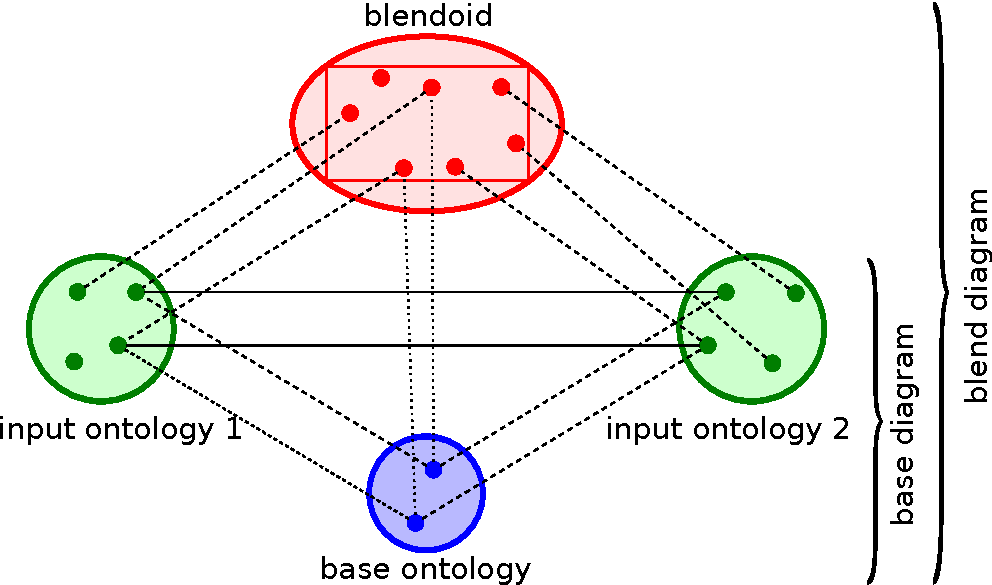
\includegraphics[width=.6\textwidth]{basic-diagram-blending}
        \caption{The basic integration network for blending: concepts in the base ontology are first refined to concepts in the input ontologies and then selectively blended into the blendoid.}%\vspace{-7mm}
        \label{fig:basic-diagram-blending}
\end{figure*}

%\smallskip
%\noindent


An \defsty{\OWL signature} consists of sets of class names, role names, and individual names. An \defsty{\OWL signature
morphism} between two \OWL signatures consists of three mappings between
the respective sets. \OWL sentences over a given signature $\Sigma$
are defined as in \cite{DBLP:conf/kr/HorrocksKS06}, e.g., 
subsumptions between classes, role hierarchies, and instances of classes
and roles, etc. \OWL models provide a domain of individuals and interpret
classes as subsets, roles as binary relations, and individuals as elements
of the domain. Satisfaction of sentences in a model is defined
in a standard way, see \cite{DBLP:conf/kr/HorrocksKS06} for details.
Moreover, given a signature morphism $\sigma:\Sigma_1\to\Sigma_2$
and a $\Sigma_2$-model $M_2$, the \defsty{reduct} $M_2\forget\sigma$
is the $\Sigma_1$-model that interprets a symbol by first translating
it along $\sigma$ and then looking up the interpretation in $M_2$.

On top of this, we define the language ${\hOWL}$ and its model-theoretic
semantics as follows.\footnote{The definition of \hOWL as given here corresponds essentially to the fragment of the distributed ontology language \DOL that homogeneously uses \OWL modules. The full \DOL language however comprises several additional features, and supports a large number of ontology languages, see \cite{DOLsemantics} for a presentation of the full semantics.}
A \hOWL ontology $O$ can be 
\begin{itemize}
\item a \defsty{basic} \OWL theory $\langle\Sigma,\Gamma\rangle$;
 $\Sigma$ is a signature, $\Gamma$ a set of $\Sigma$-sen\-tences, 
with
$\Mod(\langle\Sigma,\Gamma\rangle)$ containing all
$\Sigma$-models satisfying $\Gamma$;
\item a \textbf{translation}, written $O \textbf{ with } \sigma$, (where $\sigma:\Sigma_1\to\Sigma_2$) with \newline
$\Mod(O \textbf{ with } \sigma)=\{M\in\Mod(\Sigma_2)\ \,|\ M\forget\sigma\in\Mod(O)\}$;
\item a \textbf{union}, written $O_1 \textbf{ and } O_2$, of ontologies over the same
signature, with $\Mod(O_1 \textbf{ and } O_2)=\Mod(O_1)\cap\Mod(O_2)$\footnote
{Unions over different signatures can be modelled using translations.};
\item a \textbf{hiding}, written $O \textbf{ hide } \sigma$, with \newline $\Mod(O \textbf{ hide } \sigma)=\{M\forget\sigma \,|\ M\in\Mod(O)\}$.
\end{itemize}
A \hOWL library statement can be
\begin{itemize}
\item an ontology definition \textbf{ontology }$O\_NAME$ = $O$; or 
\item a interpretation, written \textbf{interpretation }$INT\_NAME$ : $O_1$ to $O_2$ = $\sigma$.
\end{itemize}
An interpretation is \defsty{correct}, if $\sigma$ is a theory morphism
from $O_1$ to $O_2$, that is, for every $O_2$-model $M_2$, its reduct
$M_2\forget\sigma$ is an $O_1$-model. This definition provides 
a structural approach in \hOWL, that can be compared with
instantiation of type variables in Haskell and type casting in OBJ3.

Since in some blends, not the whole theory can be mapped, Goguen
\cite{Goguen99} introduces partial signature morphisms.  Here, we follow a
common idea in category theory and model partial theory morphisms 
$\sigma :  T_1\parrow T_2$ as
spans 
%\begin{diagram}T_1 & \lTo^{\sigma_-}&dom\ \sigma&\rTo^{\sigma_+}&T_2\end{diagram} 
of ordinary (total) theory morphisms satisfying a well-definedness
condition; this has the advantage of
keeping the theory simple. $\sigma_-$ is the inclusion of $dom\ \sigma$ (the
domain of $\sigma$) into $T_1$, while $\sigma_+$ is the action of the partial
theory morphism. 
If $\sigma_-$ is an isomorphism, we say
that $\sigma$ is total, it can then be identified with the ordinary morphism
$\sigma_+\circ\sigma_-^{-1}:T_1\to T_2$:
%\begin{diagram}T_1 & \rTo^{\hspace{-1em}\sigma_-^{-1}}&dom\
  %\sigma&\rTo^{\sigma_+}&T_2\end{diagram} 
  The well-definedness
condition for partial theory morphisms $\sigma:T_1\parrow T_2$ is
similar to but more general than that for ordinary theory morphisms:
for each $T_2$-model $M_2$, its reduct $M_2\forget{\sigma_+}$ must be 
``somehow'' a $T_1$-model. The ``somehow'' can be made precise as follows:
for each $T_2$-model $M_2$, there must be a $T_1$-model $M_1$ such that
$M_1\forget{\sigma_-}=M_2\forget{\sigma_+}$. Equivalently,  
$\sigma_+:(T_1\textbf{ hide } \sigma_-) \to T_2$ is an ordinary theory
morphism (note that the models of $T_1\textbf{ hide } \sigma_-$
are precisely those models that are $\sigma_-$-reduct of some $T_1$-model).


We now recall some notions from category theory, see
\cite{AHS,zimmermann-fois} for further details.  A \defsty{diagram}
$D$ consists of a graph of ontologies $(D_i)_{i\in |D|}$ and total
theory morphisms $(D_m:D_i\to D_j)_{m\in D}$ among them.  Partial
theory morphisms can easily be dealt with: diagrams just get a little
larger when spans are used. For a diagram $D$, a \defsty{partial sink}
consists of an ontology $O$ and a family of partial theory morphisms
$(\mu_i:D_i\parrow O)_{i\in |D|}$. A \defsty{sink} is a partial sink
consisting of total morphisms only.  A partial sink is an epi-sink, if
$f\circ(\mu_i)_-=g\circ(\mu_i)_-$ for all $i\in |D|$ implies $f=g$.  A
partial sink is \defsty{weakly commutative} if all emerging triangles
commute weakly, i.e., for all $m:i\to j\in D$,
we have that $D_m\circ\mu_i=\mu_j$ as partial morphisms. Such compositions
of partial morphisms are obtained by pullback:
%\begin{diagram}
%     &&                && dom(\theta\circ\sigma)  &&             &&     \\
%    & (\theta\circ\sigma)_-&\ldLine(2,1)& \ldDotsto          &                        & \rdDotsto&            \rdLine(2,1) & (\theta\circ\sigma)_+&     \\
%  \ldTo(1,3)  & & dom\ \sigma     &&                        && dom\ \theta &&     \rdTo(1,3) \\
%    & \ldTo^{\sigma_-} && \rdTo^{\sigma_+} &                        &\ldTo^{\theta_-}&             &\rdTo^{\theta_+}&     \\
%T_1 &&                 &&          T_2           &&             && T_3 \\
%%T_1 & \rTo^{\hspace{-1em}\sigma_-^{-1}}&dom\
%%  \sigma&\rTo^{\sigma_+}&T_2
%\end{diagram} 
  For total sinks, weak commutativity amounts to ordinary
commutativity; the sink in this case is called a \defsty{co-cone}.  A
co-cone is a \defsty{colimit}, if it can be uniquely naturally
embedded into any co-cone (hence, it can be seen as a minimal
co-cone). \cite{AHS} also show that colimits are epi-sinks.

%\oliver{introduce: ontological base diagram; input ontologies; base ontologies; define `classical base diagram'}
%%	
%\begin{definition}[Diagrams, Colimits]
% ...
%\end{definition}

We now give a general definition of ontological blending capturing the
basic intuition that a blend of input ontologies shall partially
preserve the structure imposed by base ontologies, but otherwise be an
almost arbitrary extension or fragment of the disjoint union of the
input ontologies with appropriately identified base space terms. 

\begin{definition}[Ontological Base Diagram]
An \defsty{ontological base diagram} is a diagram $D$ for which the minimal nodes 
$(B_i)_{i\in D_{min}\subseteq |D|}$ are called \defsty{base ontologies},
 the maximal nodes $(I_j)_{j\in D_{max}\subseteq |D|}$ called \defsty{input ontologies}, and where the partial theory morphisms $\mu_{ij}:B_i\parrow I_j$ are the  \defsty{base morphisms}. 
If there are exactly two inputs $I_1$, $I_2$, and one base \base, the diagram $D$ is called \defsty{classical} and has the shape of a V (for total morphisms) or W (for partial morphisms). In this case, \base is also called the \defsty{tertium comparationis}. 
\end{definition}


%It defines a base ontology $O_b$, also called the tertium  comparationis, two input ontologies $O_1$ and $O_2$, and two  (possibly partial; in this case, the diagram has form W)  theory morphisms $\mu_1:O_b\parrow O_1$ and  $\mu_2:O_b\parrow O_2$ from the base ontology to the input ontologies. 
%The input ontology may define thematically overlapping domains and may thus be aligned with each other 

The basic, i.e., classical, case of an ontological base diagram with total morphisms is illustrated in the lower part of Fig.\ \ref{fig:basic-diagram-blending}. In general, however, ontological blending can deal with more than one base and two input ontologies. \cite{Coulson2001}, for instance, discusses the example of blending the input domains \emph{politics}, \emph{American culture}, and \emph{sports}, in order to create the metaphor ``He's a guy who was born on third base and thinks he hit a triple.'' \cite[p. 172]{Coulson2001} (a criticism of George Bush).
%\oliver{Examples for blending: 3 inputs with 1 base; 2 inputs with 2 bases, or some such.}

\begin{definition}[Ontological Blendoid]
  Let $D$ be a base diagram. % of ontologies and theory morphisms, also
%  called tertium comparationis. 
  A \defsty{blendoid} \blend for $D$ is a
  partial sink of \emph{signature morphisms} over $D$. A blendoid is
  called
%\vspace{-3mm}
\begin{itemize}
\item \defsty{axiom-preserving}, if the signature morphisms of
the partial sink are all theory morphisms;
\item \defsty{closed}, if it is a (partial) epi-sink (which basically means
 that the blend is generated by the diagram), otherwise \defsty{open};
\item \defsty{total}, if the partial sink is a sink;
\item \defsty{commutative}, if it is (weakly) commutative;
\item \defsty{strict}, if it is a colimit (colimits are always epi-sinks, so closed).
\end{itemize}
\end{definition}
%
Here, axiom preservation, totality and commutativity can also hold
to a certain degree. Consider the percentage of: signature morphisms
that are theory morphisms (resp.\ total); and diagrams that commute.%, which we will discuss further in the next section.

Further note that an axiom-preserving strict blend where the base diagram has
the form of a V and the base ontology is just a signature is nothing else but a $\Va$-alignment.  
Note that open blends might additionally import ontologies with new relevant
signature.

Two crucial aspect of blends are (1) morphisms within the base diagram
as well as into the blend diagram can be partial, and (2) the structure of the
blend might partially violate the shared structure of the inputs
(`violation of structure mapping').

In practice, open blends will typically be constructed by first
generating a closed blend, and then subsequently aligning this
with a new (thematically related) input ontology. In particular,
this construction can be applied by aligning two different closed
blends $\blend_1$ and $\blend_2$ obtained through the same base space
\base (here new signature elements can be created in the new colimit).
For instance, we can align the blended ontologies for
$\con{BoatHouse}$ and $\con{HouseBoat}$ by introducing houseboats as 
residents of boathouses. This
\defsty{completion} by alignment or import can be seen as an
analogue to the `running of the blend' as it is discussed in
conceptual blending \cite{FauconnierTurner2003}.

%\oliver{fix terminology with respect to Goguen's...} 

Clearly, unless we construct a strict blendoid with a rather `strong' base ontology, due to partiality there will always be exponentially many possibilities for the blend. Moreover, there are obviously infinitely many open blends regardless of partiality and the structure of the base.  
%
For instance, in the \con{House} and \con{Boat} blending formalised in \cite{goguenharrell10}, there are, in our terminology, 48 blendoids over a fixed base diagram that are axiom preserving, commutative   and closed.\footnote{Note that this differs from the (slightly inconsistent) terminology in \cite{goguenharrell10}.}

 %blendoids satisfying certain optimality principles; closedness is not explicitly mentioned but needs to come in somehow in order to get only finitely many blends. \oliver{Till: Check?} \till{if I collect what Goguen and Harrell say: ``axiom preserving, commutative and optimal w.r.t.\ degree of commutativity, degree of constant preservation,  and amount of type casting for constants.'' blendoids are always commutative and thus are of course already optimal w.r.t.\ commutativity. Closedness is not mentioned but must be somehow there.}---of these, only very few are commutative\till{really? on p.156 Goguen and Harrell define a blendoid to be always commutative}. But there are already 736 where some axoms are omitted  (that they consider ` less perspicuous'). In this blend, strict structural preservation corresponds well to `menaningful' blends, but this can be considered mostly coincidental.

% `Computing' the base space: how far did Goguen et al get? TM: when thy obtained these many blendings, was this due to many different bases/mappings,
%or due to many different cocones/colimits? TM: due to the cocones, I think. 
%They say: 
%``the algorithm computes 48 blends where every axiom is preserved, and 
%736 that fail to preserve some axioms.'' and these are obviously all
%over the same base ``V'' --- otherwise, they would get many more.
%Hence, I conclude that they cannot compute the base space.


%- estimation for combinatorial explosion in different cases (future work)?

%TODO 

%- detailed (inline) discussion on how the formal definitions capture the basic intuitions of (ontological) blending.




%
%TODO: what does this mean in the OWL-CD case??? 
%
\weg{
Work by Goguen and Harrell: 
%\subsection{Semiotic (Poetic) Blending by Goguen}\label{poems}

Semiotic Morphisms: \url{http://cseweb.ucsd.edu/~goguen/papers/sm/smm.html}

Computational Narratology \url{http://cseweb.ucsd.edu/~goguen/projs/narr.html}

Define \defsty{semiotic system} (\cite{goguenharrell10}) = algebraic theory (declaration of sorts and operations) + \defsty{level ordering} on sorts (with a top sort) + priority ordering on sorts at each level.

%\begin{task}
%        What is the relationship between a level ordering on sorts and a taxonomy?
%\end{task} 
}
%

%\begin{figure}[t]
%        \centering
%\includegraphics[width=.3\textwidth]{houseboat.png}
%\caption{House + Boat: Two Different Blends of Two Input Spaces}
%       \label{fig:goguenblend}
% \end{figure}


%%%%%%%%%%%%%%%%%%%%%%%%%%%%%%%%%%%%%%%%%%%%%%%%%%%%%
\section{Computational and Representational Challenges}\label{sec:Computational and Representational Challenges} % in Ontological Blending}
%%%%%%%%%%%%%%%%%%%%%%%%%%%%%%%%%%%%%%%%%%%%%%%%%%%%%

Conceptual blending has been proposed as a possible solution to get a handle on the notion of  computational creativity \cite{Pereira07}. The most sophisticated implementation to date related to blending probably is the tool described in \cite{goguenharrell10} for the automated generation of poems. To create similar tools specifically dedicated to the realm of ontology, we have to address at least the following three issues:
%
\begin{enumerate}
	\item The representational layer for blending needs to be specialised to ontology languages, in particular to one-sorted languages such as \OWL, and languages such as Common Logic\footnote{See \url{http://common-logic.org/}}.
	\item Given a couple (or a finite number of) ontologies, strategies are required to compute (rather than assume or handcraft) the common base ontology together with corresponding morphisms. 
	\item Given an ontological base diagram, techniques and heuristics are required that select interesting or useful blendoids according to genuine ontological principles. In particular, this requires new ranking and optimality principles.
\end{enumerate}
%

We have addressed the first item already in the previous section: the language \hOWL allows for a structured specification of blend diagrams. Note that, more generally, mixed blend diagrams can be specified in the \DOL language combining, besides several other ontology languages, first-order and \OWL ontologies (see \cite{hyper2010}). 
%
%\smallskip
%\noindent
We next briefly discuss items 2.\ and 3.\

%%
%\subsection{Blending for Ontology Languages}
%%
%

%\noindent
%\textbf{Blending for Ontology Languages.} \quad 
%As Goguen and Harrell \cite{goguenharrell10} point out, in a blending, not all properties need be preserved. In our case, the views into BoatHouse do not preserve all properties. As  Resident$\_$Boat is mapped to User, the views require  Resident$\_$Boat to be a subclass of Person, which is in fact not the case. Its reason is that the personification of the boat as a person is made available by the view, but it is not present in the target ontology. This is appropriate here, as this personification is a (local) blending principle that should not find its ways into the ontology.


%%
\subsection{Computing the Tertium Comparationis}
%%

%\smallskip
%\noindent
%\textbf{Computing the Tertium Comparationis.} \quad 
To find candidates for base ontologies that could serve for the generation of ontological blendoids, much more shared semantic structure is required than the surface similarities that alignment approaches rely on.  
The common structural properties of the input ontologies that are encoded in the base ontology are  typically of a more abstract nature. The standard example here relies on \emph{image schemata}, such as the notion of a \emph{container} mentioned earlier (see also \cite{Kuhn02}). Thus, in particular, foundational ontologies can support such selections. In analogical reasoning, `structure' is (partially) mapped from a source domain to a target domain \cite{forbus89,schweringEtAl09}. Intuitively, then, the operation of computing a base ontology can thus be seen as a bi-directional search for analogy. 

\noindent
We briefly discuss three promising candidates for this operation:
%Of course, the definition of base space that is given by this operation is rather strict, and quite unlike the notions of \emph{family resemblance} and similarity that is common in blending when applied to metaphor \cite{lakoffturner89}.
%
%\begin{quotation}
%	In every basic metaphor, the mapping preserves generic-level structure. In particular, if one takes the portion of the source domain  that is mapped and the portion of the target domain it maps onto, they will have the same generic-level structure [\ldots] The preservation of generic-level structure is, we believe, at the heart of metaphorical imagination, whether poetic or ordinary. (\cite{lakoffturner89}, p.\ 83)
%\end{quotation}	
%
%\noindent
%\textbf{Three candidate approaches:}
%

%\begin{itemize}
%	\item 
(1) \defsty{Ontology intersection:} \cite{normann08} has studied the automatisation of theory interpretation search for formalised mathematics, implemented as part of the Heterogeneous Tool Set (\Hets, see below). 
\cite{kutznormann09} applied these ideas to ontologies by using the ontologies' axiomatisations for finding their shared structure. Accidental naming of concept and role names is deliberately ignored and such names are treated as arbitrary symbols (i.e., any concept may be matched with any other). By computing mutual theory interpretations between the inputs, the method allows to compute a base ontology as an \emph{intersection} of the input ontologies together with corresponding theory morphisms. While this approach can be efficiently applied to ontologies with non-trivial axiomatisations, lightweight ontologies are less applicable, e.g., `intersecting' a smaller taxonomy with a larger one clearly results in a huge number of possible taxonomy matches \cite{kutznormann09}. In this case, the following techniques are more appropriate. 

%Yet, this also implies that the approach is more likely to succeed `the more structure' the two ontologies share: in case there is an interesting semantic (axiomatic) overlap between two ontologies, this method is more likely to succeed to provide base ontologies allowing also for potentially interesting blendoids than in the case of ontologies sharing little axiomatically.  In the latter case, the following techniques are more applicable. 

(2) \defsty{Structure-based ontology matching:} \cite{RitzeMSS08} address the problem that matching and alignment approaches are typically restricted to find simple correspondences between atomic entities of the ontology vocabulary. %A restriction that renders standard alignment techniques also useless for blending. 
They define a number of \emph{complex correspondence patterns} that can be used together with standard alignments in order to relate complex expressions between two input ontologies. For instance, the `Class by Attribute Type Pattern' may be employed to claim the equivalence of the atomic concept \con{PositiveReviewedPaper} in ontology $O_1$ with the complex concept \con{\exists  hasEvaluation . Positive} of $O_2$. Such an equivalence can be taken as an axiom of the base ontology; note, however,  that it could typically not be found by intersecting the input ontologies. Giving such a  library of design patterns may be seen as a variation of the idea of using image schemata.
	
(3) \defsty{Analogical Reasoning:} %As argued above, computing a base ontology can be modelled as a variant of analogical reasoning: a bi-directional analogy may be seen as the  computation of a common generalisation of the input ontologies. 
\emph{Heuristic-driven theory projection} is a logic-based technique for analogical reasoning that can be employed for the task of computing a common generalisation of input theories.  \cite{schweringEtAl09} establish an analogical relation between a source theory and a target theory (both first-order)  by computing a common generalisation (called `structural description'). They implement this by using anti-unification \cite{plotkin70}. A typical example is to find a generalisation (base ontology) formalising the structural commonalities between the Rutherford atomic model and a model of the solar system. This process may be assisted by a background knowledge base (in the ontological setting, a related domain or foundational ontology). Indeed, this idea has been further developed in \cite{MartinezEtAL2011}. %It remains to be seen, however, how effective these methods are for less expressive languages such as \OWL. 

%\begin{quotation}
%	A last point concerns the transfer of knowledge from the source to the target domain. In the Rutherford example, this is the projection of $\alpha_5$ to the target domain governed by the analogical relation computed so far. Such projections allow to creatively introduce new concepts on the target side. The importance of these transfers for modeling creativity and productivity cannot be overestimated.
%\end{quotation}

%Compare also the work of \cite{SwarupSylvian06,KlenkForbus09}.

%\end{itemize}

%\oliver{someone check all of the above for sanity... shorten?}

%%
%\subsection{Selecting the Blendoids: Optimality Principles}% in Ontology}
%%

%\smallskip
%\noindent
\subsection{Selecting the Blendoids: Optimality Principles} %\quad % in Ontology} 
%\oliver{clean up, re-arrange, expand}
Having a common base ontology (computed or given), there is typically a large number of possible blendoids. For example, even in the rather simple case of combining \con{House} and \con{Boat}, allowing for blendoids which only partially maintain structure (called \emph{non-primary} blendoids in \cite{goguenharrell10}), i.e., where any subset of the axioms may be propagated to the resulting blendoid, the number of possible blendoids is in the magnitude of 1000. 
%
Clearly, from an ontological viewpoint, the overwhelming majority of these candidates will be rather meaningless. A ranking therefore needs to be applied on the basis of specific ontological principles. In conceptual blending theory, a number of \defsty{optimality principles} are given in an informal and heuristic style \cite{FauconnierTurner2003}. While they provide useful guidelines for evaluating natural language blends, they do not suggest a direct algorithmic implementation, as also analysed in \cite{goguenharrell10}. Moreover, the standard blending theory of \cite{FauconnierTurner2003}  does
not assign types, which might make sense in the case of linguistic blends where type information is often ignored.  A typical example of a type mismatch in language is the
operation of \emph{personification}, e.g., turning a boat into an
`inhabitant' of the `boathouse'.  However, in the case of blending in mathematics or ontology, this loss of information is often rather unacceptable: to the opposite, a fine-grained
control of type or sort information is of the utmost importance here. 
%

Optimality principles for ontological blending will be of two kinds. (1) purely  \emph{structural/logical principles}: as introduced in Sec.~\ref{blendingintro}, these will extend and refine the criteria as given in \cite{goguenharrell10}, namely \defsty{degree of commutativity} of the blend diagram, \defsty{type casting} (preservation of taxonomical structure), \defsty{degree of partiality} (of signature morphisms), and \defsty{degree of axiom preservation}. The relative ranking and importance of these metrics, however, will remain a case-by-case decision. In the context of \OWL, typing needs to be replaced with preservation of specific axioms encoding the taxonomy.  (2) \emph{heuristic principles}:  unlike the categorical modelling of alignments, blendings can often not be adequately described by a pushout operation. Some diagrams may not commute, and a more fine-grained control is required. This particularly explains why Goguen uses $3/2$ pushouts to specify blending \cite{Goguen99}.  Generalising blendoids to be $3/2$ pushouts allows for the integration of certain optimality principles in the blending process, namely an ordering of morphisms allowing to specify their quality (for instance in terms of their degree of partiality and type violation). Essentially, this introduces preference orders on possible morphisms, which can further be regulated by specific ontological principles.  One candidate for regulating such preference orders, extending the purely structural optimality principles, would be adherence to the OntoClean methodology \cite{ontoclean02}. 



%%
%\subsection{Tool Support}
%%

%Although alignment and blending are both based on pushouts, there are two main differences:
%\begin{enumerate}
%\item Blending is a local creative construction, and the identifications
%made in the blending diagram are intended to stay local and not intended
%to influence the ontology globally. By contrast, alignment
% is a global construction on ontologies.
%\item Often, blending is not a pushout: some diagrams may not commute,
%  and a more fine-grained control is required. This particularly
%  explains why Goguen uses $3/2$ pushouts to specify blending
% \cite{Goguen99}.  Generalising blendoids to be $3/2$ pushouts allows
% for the integration of certain optimality principles in the blending
%  process, and an ordering of morphisms allows to specify their
% quality (in terms of definedness, all concepts are mapped and typing
%  is not violated). In the context of \OWL, typing needs to be
%  replaced with preservation of axioms.
%\end{enumerate}

\smallskip
\noindent
\textbf{Existing Tool Support.} \quad 
%
For carrying out blending experiments using \OWL, we use the  \hOWL language and the Heterogeneous Tool Set \Hets  \cite{MossakowskiEA06} which provides a prototypical implementation of the full \DOL language.\footnote{\Hets is available under
\url{www.dfki.de/cps/hets}. For more information on \DOL and the ISO standardisation effort OntoIOp visit \url{http://ontolog.cim3.net/cgi-bin/wiki.pl?OntoIOp}}  \hOWL allows for writing \OWL
ontologies using Manchester syntax \cite{HorridgePatelSchneider2008}
(hence they can also be imported from common tools like
Prot\'{e}g\'{e}), and \hOWL provides \emph{interpretations} in the style of OBJ views
that relate logical theories (here: \OWL ontologies), using
interpretations of theories.  Interpretations are also used to build up the
blending diagrams. Moreover, \Hets can compute colimits of such diagrams, as well as approximations of co-limits in the case where the input ontologies live in different ontology languages \cite{CodescuEtAl08}. These features are essential for the implementation of the example discussed next.


